\documentclass{article}
%\usepackage[total={6.5in,9in},centering]{geometry}
%\usepackage{amsmath}
\usepackage{college-math-j}
%\usepackage{graphicx} % for png figures
\usepackage{subcaption} % for subfigures
\usepackage{xfrac} % for sfrac (slanted inline fractions)
%\usepackage{hyperref}
\usepackage[super]{nth}
\usepackage[yyyymmdd]{datetime}
\renewcommand{\dateseparator}{-}
%\usepackage{amsaddr} % addresses up front
%\usepackage{amssymb, amsmath, bm, nameref}
%\pagenumbering{gobble} % no page

\theoremstyle{theorem}
\newtheorem{theorem}{Theorem}

\theoremstyle{definition}
\newtheorem*{definition}{Definition}
\newtheorem*{remark}{Remark}

%\newcommand{\SETb}{SET\texttrademark\ } % this one has a space after
\newcommand{\SET}{{\em SET}}
\newcommand{\SETs}{{\em SET}s}

\newcommand{\SETSET}{{\sc setset}}
\newcommand{\SETSETb}{{\sc setset }}
\newcommand{\SETSETA}{{\sc setset-all}}
\newcommand{\SETSETAb}{{\sc setset-all }}
\newcommand{\ED}{{\sc enumerate\_deals}}
\newcommand{\EDb}{{\sc enumerate\_deals }}


\begin{document}


\title{Enumerating Deals in the Game of SET}
\author{Reuben Settergren}
%\email{rjs@jhu.edu}

\thanks{Thanks to Liz McMahon and Gary Gordon of Lafayette College for helpful
  correspondence during the development of this capability, as well as for
  writing the delightful book {\em The Joy of Set} \cite{JOS}.}

\thanks{Thanks also to the 6-\nth{7} grade Math Discovery Club at The Cambridge
  School ({\tt cambridgeclassical.org}), who set me off on this journey.}

\maketitle


\section{What are the chances?}
How often, when playing a game of SET\texttrademark, are you faced with a
difficult opening deal of 12 cards? Is it really necessary to deal out another 3
(or 6, or \ldots) cards? Or could one or more \SETs\footnote{A note on
terminology: SET will refer to the card game, `\SET' will refer to three cards
that meet the criteria for removal according to the rules of the game, and `set'
will take its normal mathematical sense of an unordered collection. A $k$-set
(or for instance 5-set or 12-set) will refer to a set of $k$ cards.} be hiding
in those initial 12, to be found with further patient searching?  ``What are the
chances,'' we all wonder, ``that an initial deal has no \SET?'' Or how about
exactly 1 \SET? What is the mean number of \SETs~in an initial deal, or what if
the game were changed to start with 9 cards? The beauty of SET is that it
stimulates all sorts of lines of mathematical inquiry.


\section{Background}
In the card game SET, each card depicts 4 attributes (number, texture, color,
shape), and each attribute has 3 possible values, for a total of $3^4=81$
cards. A \SET~is defined as a set of 3 cards for which all attributes are
either all the same, or all different. A fundamentally important fact about
\SETs~is that, for any two distinct cards, there is a unique third card which
completes a \SET~with them. The unique \SET-mate of any two cards can be
constructed by setting all four attributes appropriately: if the first two cards
have the attribute the same, set the third the same; if they are different, set
the third card's attribute different.

The rules of SET specify that a game begins by dealing 12 cards, and additional
groups of 3 as long as \SETs~cannot be found. So the question naturally arises,
what is the probability that 12 cards have no \SET?  The instructions that come
with SET \cite{SET} state that ``There are $\sim 33:1$ odds that a \SET~is
present in 12 cards, and \mbox{$\sim 2500:1$} odds when 15 cards are on the
table,'' i.e. probabilities of $\sim 1/34\sim 2.94\%$ (or perhaps they intended
$1/33\sim 3.03\%$) and $\sim 1/2501\sim 0.04\%$, respectively. In the delightful
book {\em The Joy of Set} (\cite{JOS} ch 10), McMahon and Gordon use a computer
simulation to sample 100 million deals, and encountered 3,228,460 \SET-less
deals (3.22846\%), and report that this larger number is consistent with online
reports of other simulations. But these approximate results, while practically
useful, only whet the mathematician's appetite for exact answers.

\section{Sets without \SETs}
Before the game of SET was invented it was known (in equivalent form in the
field of Affine Geometry \cite{MAXCAP}) that the maximum number of cards with no
\SET~is 20. So if hapless players keep dealing 3 more cards until they can't
find a \SET~in 21 cards, they should look harder!  Knowing this limit, Donald
Knuth \cite{SETSET}, \cite{SETSET-ALL} used a computer to efficiently calculate
the number of \SET-less $k$-sets for $k\leq 21$. The efficiency of Knuth's
solution relied on {\em isomorph rejection}. To illustrate this, let's adopt
Knuth's abbreviated notation for SET, where cards are indicated as
4-vectors. Each of the 4 coordinate dimensions represents one attribute (number,
texture, color, shape), and the digits 1,2,3 represent the 3 possible values of
that attribute. Thus the deck is represented by the 81 vectors (1,1,1,1),
(1,1,1,2), (1,1,1,3), (1,1,2,1), \ldots (3,3,3,3).

Two sets of cards are isomorphic if there is a rotation of attributes/values
that maps one into the other. Knuth provides a specific example:
\begin{quotation}For example the set $\{(1,2,2,3), (2,2,3,3)\}$ is
  isomorphic to the set $\{(1,1,1,1),$ $(1,1,2,2)\}$, because we can interchange
  coordinates 1 and 4, then map $3\mapsto 1$ in coordinate~1, $2\mapsto1$ in
  coordinate~2, and $(2,3)\mapsto(1,2)$ in coordinate~3.
\end{quotation}
One step at a time, this transformation sequence looks like this (all of the
intermediate results are also isomorphic to the starting set):
\begin{align*}
(\text{starting 2-set)\hspace{5mm}}&  \{(1,2,2,3), (2,2,3,3)\}  \\
  (\text{swap coords 1, 4})  \rightarrow & \{(\mathbf{3},2,2,\mathbf{1}), (\mathbf{3},2,3,\mathbf{2})\} \\
  (\text{map coord 1:~} 3\mapsto 1)\rightarrow & \{(\mathbf{1},2,2,1), (\mathbf{1},2,3,2)\} \\
  (\text{map coord 2:~} 2\mapsto 1)\rightarrow & \{(1,\mathbf{1},2,1), (1,\mathbf{1},3,2)\} \\
  (\text{map coord 3:~} (2,3)\mapsto(1,2))\rightarrow & \{(1,1,\mathbf{1},1), (1,1,\mathbf{2},2)\}
\end{align*}


The `secret sauce' of Knuth's program (called \SETSET) is the realization that,
once any specific set is determined to have a \SET~or not, all sets which are
isomorphic have the same number of \SETs. As Knuth notes, ``There are $4! \times
3!^4 = 31104$ isomorphisms, since we can permute the coordinates [attributes] in
4! ways and we can permute the individual values of each coordinate position in
3! ways.''  Thus counting the number of isomorphic \SETs~all at once can save a
lot of time compared to a complete enumeration.

Consider the trivial questions, ``How many 1-sets or 2-sets are \SET-less?''
Knuth's program arrives at the obvious answer of ``all of them''
($\binom{81}{1}=81$ for $k=1$ and $\binom{81}{2}=3240$ for $k=2$) not by
enumerating all $k$-sets and testing each one, but by testing only one per
isomorphism group. All 81 1-sets are isomorphic to ${(1,1,1,1)}$, so the answer
for $k=1$ requires only 1 test. 2-sets fall into 4 isomorphism groups, which are
represented by these 2-sets:
\begin{itemize}
\item $\{(1,1,1,1), (1,1,1,2)\}$ (isomorphism group size: 324)
\item $\{(1,1,1,1), (1,1,2,2)\}$ (isomorphism group size: 972)
\item $\{(1,1,1,1), (1,2,2,2)\}$ (isomorphism group size: 1296)
\item $\{(1,1,1,1), (2,2,2,2)\}$ (isomorphism group size: 648)
\end{itemize}
Those 4 isomorphism groups can be characterized as pairs of cards for which 3,
2, 1, or 0 attributes match. (Why, combinatorially, are those isomorphism group
sizes correct?) So \SETSETb is able to count the \SET-less 2-sets by adding up
isomorphism groups for just 4 cases (324+972+1296+648=3240), rather than
enumerating all 3240.

In the same manner, \SETSETb searches all sets of size up to 21 by starting with
(1,1,1,1) and adding cards, but pruning the search tree and backtracking to try
adding a different card, whenever:
\begin{itemize}
\item Adding another card introduces a \SET, or
\item Adding another card forms a set which is isomorphic to a
  previously-accounted-for \SET-less set.
\end{itemize}
\SETSETb ends early when it is meets conditions that guarantee that all
subsequent cards are in previously-accounted-for isomorphism groups. In this
way, \SETSETb was able to count all the \SET-less sets within
$\Sigma_{k=1}^{21}\binom{81}{k}\sim 2.04\times 10^{19}$ sets, by inspecting only
514,488,889 cases, and avoiding inspection of isomorphic cases. Running \SETSETb
on my laptop takes about four and a half hours.

A few years later, Knuth improved on \SETSETb with a better program called
\SETSETA, by expanding the sense of isomorphic equivalence, yielding larger
isomorphism groups, and thus fewer representative cases to inspect. For
instance, while \SETSETb considered 73,638,164 isomorphism groups for \SET-less
sets of size $k=12$, \SETSETAb dealt with only 1437. In total, \SETSETAb dropped
the 514,488,889 isomorphism groups processed by \SETSETb to only 9606, and thus
had drastically improved speed -- reaching the same answers as \SETSETb in just
3m45s (on the same hardware).

Knuth's \SETSETb programs yield the exact answer for that SET question of first
importance, ``What is the chance that an initial deal of 12 cards has no \SET?''
The number of 12-sets with no \SET~is 2,284,535,476,080, so in combination with
the simple combinatoric fact that there are $\binom{81}{12}$ 12-sets in all, the
probability is
$$\frac{2284535476080}{70724320184700} = 3.23020\ldots\%.$$
(The estimate of 3.22846\% from $10^8$ samples (\cite{JOS}) is pretty close!)

\section{Sets with \SETs}
As satisfying as that exact answer is, Knuth's \SETSETb programs only consider
sets that have 0 \SETs. The curiosity of SET-playing mathematicians (or without
loss of generality, all mathematicians!) naturally turns to sets that do contain
\SETs. What are the chances there is just one \SET~hiding in that initial deal
of 12, vs an easier-to-find 2 (or 3 (or more))?

Let's start small (see \cite{JOS} ch 5 for the fuller combinatorial analysis of
$k=3,4,5$). For $k=3$, the only posibilities are 1 \SET~(the 3 cards {\em are}
a \SET), or 0 \SETs~(they {\em aren't}). Of the $\binom{81}{3}=85320$ 3-sets,
1080 are \SETs~(why?), thus $85320-1080=84240$ are \SET-less (\SETSETb yields
the same result in reverse: since 84240 3-sets are \SET-less, 85320-84240=1080
must have \SETs). Similarly, the $\binom{81}{4}$ 4-sets break down into 1579500
that have 0 \SETs, and 84240 that have 1 \SET.
\footnote{Did you notice that number 84240 just turned up twice? It is the
number of 3-sets {\em without} \SETs, and the number of 4-sets {\em with} a
\SET. Both times it is 78*1080, but for different reasons.  The number of
3-deals with 1 SET (the number of 3-deals which {\em are} a SET) is 
1080. But whenever two of the 81 cards are dealt, there are 79 remaining cards
-- one of which completes a SET and 78 of which do not. So the number of 0-SET
triples are 78 times as many as 1-SET triples. However, every 4-set with 1 SET
is a 3-deal with 1 SET, plus one more card. After a SET is laid out, there are
78 remaining cards which could be added to form a 1-SET 4-deal. So the number of
1-SET 4-deals is also 78 times as many as 1-SET triples.}

So for $k=3,4$, since the only possibilities are 0 or 1 \SETs, the \SET-less
counts from Knuth's \SETSETb give a complete picture. But at $k=5$, things get
more interesting. Although it would would take at least 6 cards to have two
\SETs~which are {\em disjoint}, it's possible for 5 cards to have two \SETs~that
share one card. (But it is impossible for two \SETs~to share two cards -- why?)
So although \SETSETb~tells us that 22,441,536 of the $\binom{81}{5}$ 5-sets have
0 \SETs, it doesn't tell us how the remaining 5-sets divide up between those
that have 1 \SET~or 2 \SETs. Combinatorics (\cite{JOS}, pp.~56-58) yields counts
of 3,116,880 with 1 SET and 63,180 with 2 SETs. As $k$ increases, however, so
does the complexity of combinatorial analysis, and $k=12$ is way too complex!

\section{Counting up to 12}
It would be an interesting research project (Master's thesis?) to adapt Knuth's
isomorphism rejection to also count isomorphism classes that have nonzero \SETs,
but it is more straightforward to attempt a complete enumeration. A brute-force
enumeration of all 12-card sets must consider $\binom{81}{12}$ cases (about
$7\times 10^{13}$). McMahon, Gordon et al note (\cite{JOS} p.~259) that, even
though their computer program can process about 100 million deals per hour, a
complete enumeration would still take 80 years. Enumeration, they note, ``might
be feasible with streamlined code and faster machines or parallel processing.''

As a mathematician and software engineer, my response was ``challenge
accepted!'' Given the massive parallelism of modern Graphical Processing Units
(GPUs), 70 trillion doesn't seem all that unapproachable. The program I wrote is
called \ED, and source code is available on GitHub \cite{ME}. \EDb can be run
serially, or in parallel using threads or OpenCL \cite{OPENCL} kernels. Note
that OpenCL can be configured so that its kernels can be parallelized onto
either CPU or GPU resources.

Skipping over many interesting implementation details (available in a larger
paper, also on GitHub), \EDb accomplished an exhaustive enumeration for up to 12
cards, and the results are presented in Table \ref{THE_TABLE}. Columns of the
Table are numbers of cards $k$, and rows are numbers of \SETs~found in those
$k$-\SETs.  The top row of the table (0 \SETs) matches the results of \SETSET,
so that's a vote of confidence.

\begin{table}
  \caption{Enumeration Results}\label{THE_TABLE}
  \centering
  \begin{tabular}{r | r r r r r r }
    & \multicolumn{6}{c}{Number of cards} \\
    \hline\hline
    SETs & 3 & 4 & 5 & 6 & 7 & 8   \\
    \hline
0  & 84240 & 1579500 & 22441536 & 247615056 & 2144076480 & 14587567020  \\
1  & 1080 & 84240 & 3116880 & 71772480 & 1137240000 & 12981215520 \\
2  &  &  & 63180 & 5068440 & 184485600 & 3996514080 \\
3  &  &  &  & 84240 & 11372400 & 573168960 \\
4  &  &  &  &  &  & 22744800 \\
5  &  &  &  &  & 42120 & 3032640 \\
6  &  &  &  &  &  &  \\
7  &  &  &  &  &  &  \\
8  &  &  &  &  &  & 10530 \\
\hline
$\binom{81}{N}$ & 85320 & 1663740 & 25621596 & 324540216 & 3477216600 & 32164253550  \\
\hline
seconds & 0.001 & 0.002 & 0.045 & 0.56 & 6.3 & 69 
  \end{tabular}

  \vskip 5mm

  \begin{tabular}{r | r r r r }
    SETs & 9 & 10 & 11 & 12 \\
    \hline
0  & 77541824880 & 318294370368 & 991227481920 & 2284535476080 \\
1  & 108956689920 & 676366666560 & 3091339021680 & 10266579666720 \\
2  & 56941354080 & 557948898000 & 3829696640640 & 18459179294400 \\
3  & 15417548640 & 253318946400 & 2704419900000 & 19278240770880 \\
4  & 1857807900 & 62354111040 & 1144078603200 & 12746054337120 \\
5  & 160729920 & 9176162112 & 306795509280 & 5650817178240 \\
6  & 11119680 & 827405280 & 49231877760 & 1649199670560 \\
7  & & 78848640 & 6382949040 & 330527433600 \\
8  & 758160 & 23882040 & 729349920 & 48500063820 \\
9  &  & 3032640 & 243622080 & 8323838640 \\
10 &  &  & 21228480 & 2091005280 \\
11 &  &  & & 160729920 \\
12 & 1170 & 84240 & 2611440 & 86346000 \\
13 &  &  & 379080 & 21340800 \\
14 &  &  &  & 3032640 \\
\hline
$\binom{81}{N}$ & 260887834350 & 1878392407320 & 12124169174520 & 70724320184700 \\
\hline
seconds & 646 & 5697 & 45298 & 324480
  \end{tabular}
\end{table}

The bottom row of the table is wall-clock computation time for the GPU (NVIDIA
Quadro P4000). The total time for $k=3\ldots 12$ was 104.5h=4.35d, of which
90.1h = 3.75d was required for $k=12$. (Because of combinatorial explosion, the
12-card enumeration consumed the lion's share of processing.) The 12-card
processing rate was 218M deals/second, and the overall rate was 226M/second
(\EDb is faster for smaller $k$, because fewer triples need to be checked for
each set). Single-threaded, the 12-card enumeration ran at 842K/s (projected
exhaustive enumeration time 972d=2.66y). Thus GPU processing yielded a
218M/842K$\sim$256x speedup (at least comparing the specific processors used).

One interesting feature of the table is repeated numbers. The count of 84240
shows up 4 times (as well as its half 42120), 3032640 three times, and 160729920
twice. The table is full of multiples of 1080 (the number of \SETs), and also of
1170 (the number of 9-sets with 12 SETs, aka {\em planes}, see below for more,
and \cite{JOS} for an extensive treatment of the relationship between SET and
affine projective geometry). This repetition invites questions such as, is there
a meaningful bijection between the 9-sets with 5 SETs, and the 12-sets with 11
SETs (both 160729920)? Or is the repetition just a coincidence from
combinatorial reuse of so many of the same prime factors?

One interesting question the Table can answer for us is the average number of
\SETs~per starting deal. This expected value is actually known analytically; a
clever combinatorial argument (see \cite{JOS}, pp 59-62) yields:
$$E[\text{\em SET}s}] = \frac{1080\times
    \binom{78}{9}}{\binom{81}{12}}=2.78481\ldots$$
The numerator of that fraction basically reads ``each possible \SET~(1080 of
them) and 9 more cards (of the remaining 78).'' This elegant result is obtained
without knowledge of individual probabilities of 0, 1, \ldots 14 \SETs, but it
is confirmed by computing an expected value directly from those probabilities,
from the column for $k=12$:
$$\frac{0\cdot 2284535476080 + 1\cdot 10266579666720 + \ldots + 14\cdot
  3032640}{\binom{81}{12}}$$
$$=\frac{196953803046000}{70724320184700}=\frac{220}{79}=2.78481\ldots$$

Another very obvious feature of the Table is gaps. The first gap appears in the
7 column, and from it we can see that a set of 7 cards can have 0, 1, 2, 3, or 5
SETs, but not exactly 4 SETs. There are also gaps in the 8, 9, 10, and 11-card
columns, but the 12-card initial deal has no gaps; any number of sets from 0 to
14 (the max possible for 12 cards) could occur.

The most interesting column is probably 9 cards, because of connections to
planes in affine projective geometry. A plane is 9 cards that contains 12 \SETs,
which can be arranged 3x3 so that \SETs~are horizontal, vertical, and diagonal
lines (see Figure \ref{PLANE}). A plane can be generated from any 3 cards that
are not a \SET~(just as a Euclidean plane is determined by any 3 points that are
not on the same line), by computing the closure (adding \SET-mates until every
pair's \SET-mate is present). The number of 3x3-arranged planes is $81\cdot
80\cdot 78=505440$ (two cards are chosen freely, the third card cannot be the
one that completes a set, and then the remaining six cards are
determined). Dividing out the number of 3x3 arrangements of any 9-card plane
(which is $9\cdot 8\cdot 6$ -- why?), we see that the number of planes is
$$\frac{81\cdot 80\cdot 78}{9\cdot 8\cdot 6} = 1170$$
which is confirmed in the Table at column 9, row 12.

\begin{figure}[!htb]
  \center{\includegraphics[width=0.6\textwidth]{setplanemed.png}}
  \caption{\label{PLANE}9 cards containing 12 \SETs~is arranged 3x3 and repeated
    as a tile, so that the 12 \SETs~can be seen as every horizontal, vertical
    and diagonal line. The initial arranged plane is generated from the three
    non-\SET~cards in the outlined non-collinear positions.}
\end{figure}

The situation in which 9 cards has 8 SETs, is explained by Liz
McMahon:\footnote{Co-author of \cite{JOS}, personal correspondence.}
\begin{quote}
If you take a plane [1170 possibilities] and remove one card, what's left [8
  cards] has 8 \SETs~[10530 possibilities].  You can then add another point that
doesn't complete any more \SETs~[72 possibilities -- why?], and that gives you
the 8 \SETs~in 9 cards [758160=10530*72].
\end{quote}
Between 9-card planes with 12 \SETs, and 9-sets with only 8, however, it is
impossible to have 9-sets with 9, 10, or 11 \SETs. An 8-\SET~8-set is at a
tipping point, so that any \nth{9} card that completes any \SET~also completes
three more.

Although the gaps in the Table are obvious, more subtle patterns in the data
appear when graphed, as in Figure \ref{FIGCOLS}, where each column of the Table
(deal size) is one curve.

Looking down the left side of Figure \ref{FIGCOLS}, for number of \SETs=0, we
see at the top of the stack, 3 cards has the highest probability of 0 \SETs, and
as the deal size increases, the probability of 0 \SETs~drops. These are the
results of \SETSETb up to $k=12$, rendered as probabilities rather than counts. 

The curves for deals of 3 and 4 cards have only 2 data points (0 \SETs~or 1
\SET), and larger deals extend to more possible \SETs, up to a maximum of 14
\SETs~for a 12-card deal. For that all-important 12-card curve, it is evident
that the most likely outcome is 3 \SETs~(probability
$19278240770880/70724320184700\sim 27.26\%$), and the probability of 2 \SETs~is
almost as likely. Together, 2 or 3 \SETs~constitute a little more than 50\%
probability; and the probability of 1-5 \SETs~is almost 94\%.

The vanishingly small probabilities for more than 6 \SETs~collapse all the
curves together. But the bottom half of Figure \ref{FIGCOLS} also graphs the
data in logarithmic scale, revealing additional characteristics of the data --
for instance (as discussed above), adding a \nth{9} card to an 8-\SET~8-set, and
either reaching a 12-\SET~plane, or remaining at 8 \SETs.

Gaps are apparent in log scale, as well as another interesting feature, which is
how adjacent curves `sag' into the gaps. The biggest sag is in the 12-curve at
11 \SETs, which sags into the 11-\SET~gap in the 9, 10, and 11-card
curves. Evidently, the impossibility of 11 \SETs~in fewer than 12 cards
diminishes the probability of 11 \SETs~in 12 cards. Other sags are evident above
other gaps.

\begin{figure}[!htb]
  \center{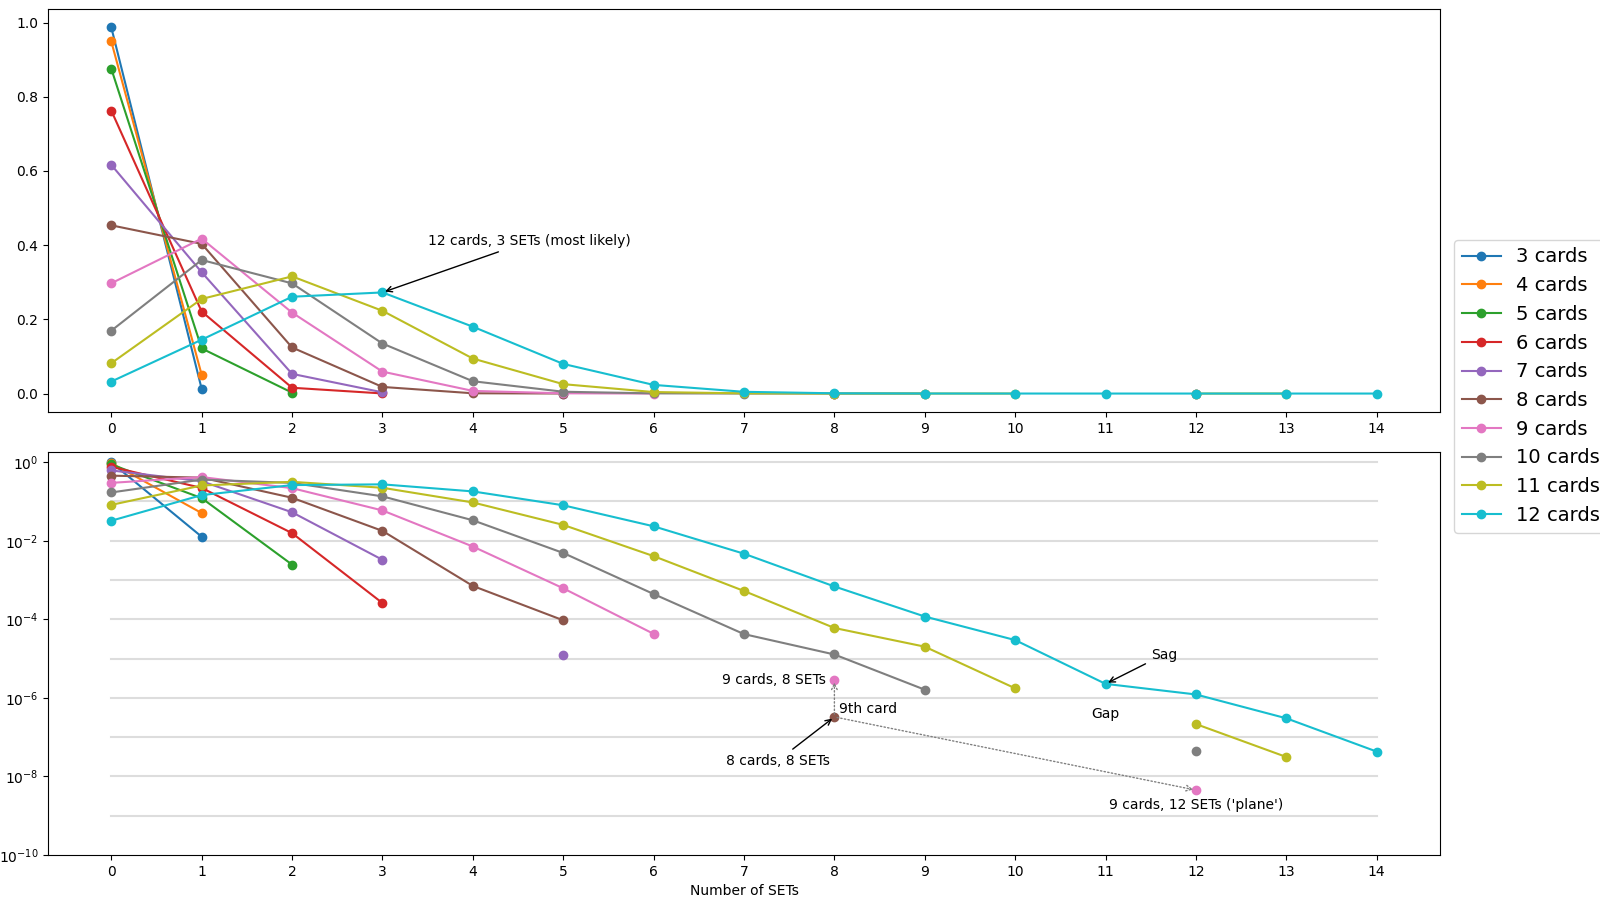
\includegraphics[width=\textwidth]{annotated.png}}
  \caption{\label{FIGCOLS} Each curve is one deal size (table column); $X$ is
    number of SETs, $Y$ is probability.}
\end{figure}

\section{Conclusion}
This paper improves on the speed of enumeration of starting deals for the card
game \SET, to accomplish exhaustive enumeration for up to 12 cards, in a little
over 4 days. As the marginal factor for extra time spent is about 7x for each
additional card, the same hardware and software could enumerate 13, 14, and 15
cards in about 1 month, 7 months, and 4 years, respectively. To reach a complete
analysis at 21 cards, computational power would have to grow by many orders of
magnitude; or an analytical or non-exhaustive enumerative solution would have to
be devised (perhaps along the lines of Donald Knuth's
isomorphism-rejection-based enumerations of the 0-\SET~problem).



\begin{thebibliography}{9} % 1-digit reference nums


\bibitem{SETSET}Knuth, Donald E., {\sc setset} (1996), Documented programs in
  CWEB, from
  \url{https://www-cs-faculty.stanford.edu/~knuth/programs/setset.w}. Accessed
  \today.

\bibitem{SETSET-ALL}Knuth, Donald E., {\sc setset-all} (2001), Documented
  programs in CWEB, from
  \url{https://www-cs-faculty.stanford.edu/~knuth/programs/setset-all.w}. Accessed
  \today.

\bibitem{JOS} McMahon, Liz, Gary Gordon, et al, 2016. {\em The Joy of SET: The
  Many Mathematical Dimensions of a Seemingly Simple Card Game}, Princeton
  University Press, Princeton NJ.

\bibitem{OPENCL} Open Computing Language (OpenCL), from {\tt
  khronos.org/opencl}, accessed \today.

\bibitem{MAXCAP}Pellegrino, G., 1971. ``Sul massimo ordine delle calotte in
  $S_{4,3}$'' [{\em The maximal order of the shperical cap in $S_{4,3}$}], {\em
  Matematiche} {\bf 25}, pp 149-157.

\bibitem{SET} SET Enterprises, Inc. \url{https://www.setgame.com}

\bibitem{ME}Settergren, Reuben, 2019. \url{https://github.com/RubeRad/SET}
  
\bibitem{VINCI}Vinci, Jim, 2009. ``The maximum number of sets for $n$ cards and
  the total number of internal sets for all partitions of the deck,'' on the
  SET game website at
  \url{https://www.setgame.com/sites/default/files/teacherscorner/SETPROOF.pdf},
  accessed \today.

\bibitem{WIKI} Wikipedia article ``Combinatorial Number System,'' \url{https://en.wikipedia.org/wiki/Combinatorial_number_system#Finding_the_k-combination_for_a_given_number},
  accessed \today.

\end{thebibliography}
 
\end{document}
